\documentclass[
  dvipdfmx
]{standalone}
\usepackage{tikz}
\usetikzlibrary{spath3}
\usetikzlibrary{knots}
\usetikzlibrary{hobby}
\usetikzlibrary{patterns}
\begin{document}
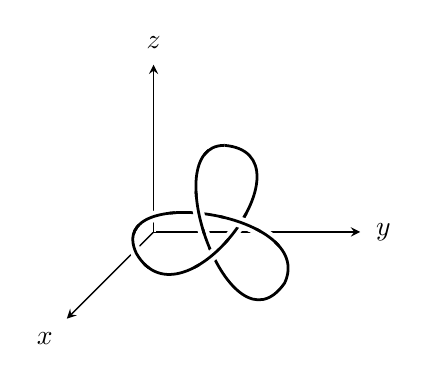
\begin{tikzpicture}
  \begin{knot}[
    consider self intersections=true,
    ignore endpoint intersections=false,
    % draft mode=crossings,
    every strand/.append style={line width=1pt},
    flip crossing=3,
    flip crossing=4,
    flip crossing=5,
    flip crossing=7,
    flip crossing=8,
    flip crossing=11,
    clip width=4,
    clip radius=6pt,
    % background color=red,
  ]
  \strand[-stealth, line width=0.5pt] (-0.7,-0.5,0) -- (2,-0.5,0) node[right] {$y$};
  \strand[-stealth, line width=0.5pt] (-0.7,-0.5,0) -- (-0.7,1.7,0) node[above] {$z$};
  \strand[-stealth, line width=0.5pt] (-0.7,-0.5,0) -- (-0.7,-0.5,3) node[below left] {$x$};
  \strand (0.2,0.6)
  %node[above right] {$\mathrm{Im}\, K$}
  .. controls +(180:0.9) and +(235:1.2) .. (-50:1.5)
  .. controls +(65:1) and +(115:1) .. (220:1.2)
  .. controls +(300:1.2) and +(-5:1.2) .. (0.2,0.6)
  ;
  \end{knot}
\end{tikzpicture}
\end{document}